\begin{center}
\underline{\Large{T.P.N°7: Flexión Compuesta Recta y Oblicua}}
\end{center}

\begin{enumerate}
\item a) Dada una columna de esbeltez reducida, que se encuentra solicitada por un momento MD = 1,5 tnm, ML = 1 tnm, ND = 75 tn y NL = 45 tn, dimensionar su sección y hallar la armadura necesaria según CIRSOC 201-05 y CIRSOC 201-82. Considerar un hormigón H-25 según Reglamento CIRSOC 201-05 y H-21 según CIRSOC 201-82.\\
b) Dibujar a escala la sección, verificando recubrimientos y separación.

\item a) Diseñar la columna de sección rectangular indicada en la Figura \ref{figura1} como C que pertenece a un edificio sometida a las siguientes cargas:\\
PD = 61 tn\\
PL = 25 tn\\
MxD = 0,7 tnm\\
MxL = 0,4 tnm\\
MyD = 1,2 tnm\\
MyL = 0,5 tnm\\
Sección tentativa\\
b = h = 30 cm\\
Efectuar los cálculos según CIRSOC 201-05 y CIRSOC 201-82. El hormigón es H-25 según CIRSOC 201-05, H-21 según CIRSOC 201-82 y el acero ADN 42/50.\\ 
b) Dibujar la sección de la viga a escala.

\begin{figure}[H]
\begin{center}
	 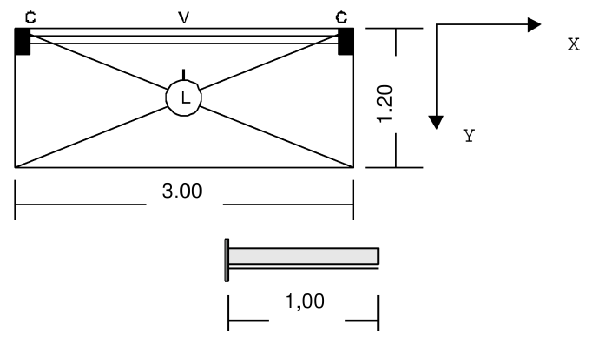
\includegraphics[scale = 0.9]{chapters/chapter_1/images/figura1.png}
     \caption{Planta de la columna correspondiente al ejercicio 2)}
     \label{figura1}
\end{center}
\end{figure}

\end{enumerate}
\newpage
\begin{center}
\underline{\Large{Solución}}
\end{center}

\begin{enumerate}
\item \underline{Diseñar una columna de esbeltez reducida según CIRSOC 201-05}

\underline{Datos:}\\
Hormigón H-25 $\Rightarrow f'c = 250 \frac{Kg}{cm^2} = 25 MPa$\\
Acero ADN 42/50 $\Rightarrow fy = 4200 \frac{Kg}{cm^2} = 420 MPa$\\
b = h = 35cm\\
Recubrimiento Cc = 2cm\\
Estribos $\phi$ 8mm\\
Diámetro de barra $\phi$ 20mm\\
$M_D = 1.5t.m$\\
$M_L = 1t.m$\\
$N_D = 75t$\\
$N_L = 45t$\\

\begin{itemize}
\item \underline{Estado de cargas}

\begin{align*}
& M_{u1} = 1.2 \cdot M_D + 1.6 \cdot M_L = 1.2 \cdot 1.5 t.m + 1.6 \cdot 1 t.m = \framebox{$3.4t.m$}\\
& M_{u2} = 1.4 \cdot M_D = 1.4 \cdot 1.5 t.m = 2.1t.m\\
& M_n = \frac{M_u}{\phi} = \frac{3.4 t.m}{0.65} = \framebox{$5.23t.m$}\\
& \\
& N_{u1} = 1.2 \cdot N_D + 1.6 \cdot N_L = 1.2 \cdot 75 t + 1.6 \cdot 45 t = \framebox{$162t$}\\
& N_{u2} = 1.4 \cdot N_D = 1.4 \cdot 75 t = 105t\\
& N_n = \frac{N_u}{\phi} = \frac{162 t}{0.65} = \framebox{$249.23t$}
\end{align*}

\item \underline{Esfuerzos reducidos}

\begin{align*}
& m_{n} = \frac{M_n}{b \cdot h^2 \cdot f'c} = \frac{5.23t.m \cdot 1000\frac{Kg}{t} \cdot 100\frac{cm}{m}}{35cm \cdot (35cm)^2 \cdot 250 \frac{Kg}{cm^2}} = \framebox{0.0487}\\
& n_{n} = \frac{N_n}{b \cdot h \cdot f'c} = \frac{249.23t \cdot 1000\frac{Kg}{t}}{35cm \cdot 35cm\cdot 250 \frac{Kg}{cm^2}} = \framebox{0.81}
\end{align*}


\item \underline{Gamma}

\begin{align*}
& \gamma = \frac{h - 2 \cdot Cc - 2 \cdot dbe - db}{h} \\
& \gamma = \frac{35cm - 2 \cdot 2cm - 2 \cdot 0.8cm - 2cm}{35cm} = 0.78 \approx \framebox{0.8}
\end{align*}

\begin{figure}[H]
\begin{center}
	 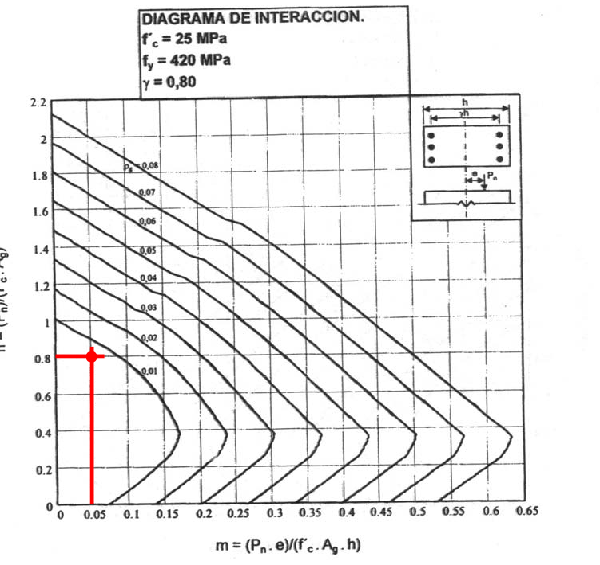
\includegraphics[scale = 0.9]{chapters/chapter_1/images/figura2.png}
     \caption{Diagrama de interacción $\gamma = 0.8$)}
\end{center}
\end{figure}
Ingresando al diagrama de interacción para 6 barras con $m_{n}=0.0487$, $n_{n}=0.81$ y $\gamma = 0.8$ tenemos $\rho \leq 0.01 \Rightarrow$ adopto $\rho=0.01$

\item \underline{Armadura}

\begin{align*}
& As_{total} = \rho \cdot b \cdot h = 0.01 \cdot 35cm \cdot 35cm = \framebox{$12.25cm^2$}
\end{align*}
Adopto 4 barras $\phi$ 20 mm con $As_{total}=\framebox{$12.56cm^2$}$\\
Adopto estribos $\phi$ 8 mm cada 20cm.\\

\item \underline{Verificación de Separaciones}\\
\\
Adopto s = 20 cm.\\
\[ s = 20cm \leq \left\{ \begin{array}{ll}
         12 \cdot db = 12 \cdot 2cm = 24cm \quad \surd &\\
         b = 35cm \quad \surd & \end{array} \right. \] 
\end{itemize}
\newpage
\item \underline{Diseñar una columna de esbeltez reducida según CIRSOC 201-82}

Hormigón H-21 $\Rightarrow \beta_R = 175 \frac{Kg}{cm^2}$\\
Acero ADN 42/50 $\Rightarrow \beta_S = 4200 \frac{Kg}{cm^2}$\\
b = h = 35cm\\
Recubrimiento r = 2cm\\
Estribos $\phi$ 8mm\\
Diámetro de barra $\phi$ 20mm\\
$M_D = 1.5t.m$\\
$M_L = 1t.m$\\
$N_D = 75t$\\
$N_L = 45t$\\

\begin{itemize}
\item \underline{Estado de cargas}

\begin{align*}
& M_{servicio} = M_D + M_L = 1.5 t.m + 1 t.m = \framebox{$2.5t.m$}\\
& \\
& N_{servicio} = N_D + N_L = 75 t + 45 t = \framebox{$120t$}
\end{align*}

\item \underline{Esfuerzos reducidos}

\begin{align*}
& m_{n} = \frac{M_{servicio}}{b \cdot d^2 \cdot \beta_R} = \frac{2.5t.m \cdot 1000\frac{Kg}{t} \cdot 100\frac{cm}{m}}{35cm \cdot (35cm)^2 \cdot 175 \frac{Kg}{cm^2}} = \framebox{0.033}\\
& n_{n} = \frac{N_{servicio}}{b \cdot d \cdot \beta_R} = \frac{120t \cdot 1000\frac{Kg}{t}}{35cm \cdot 35cm\cdot 175 \frac{Kg}{cm^2}} = \framebox{0.56}
\end{align*}

\item \underline{d1/d}

\begin{align*}
& d_1 = r + dbe - \frac{db}{2} = 2cm + 0.8cm + \frac{2cm}{2} =  \framebox{$3.8cm$}\\
& \frac{d_1}{d} = \frac{3.8cm}{35cm} = 0.11 \Rightarrow \framebox{0.10}
\end{align*}

\begin{figure}[H]
\begin{center}
	 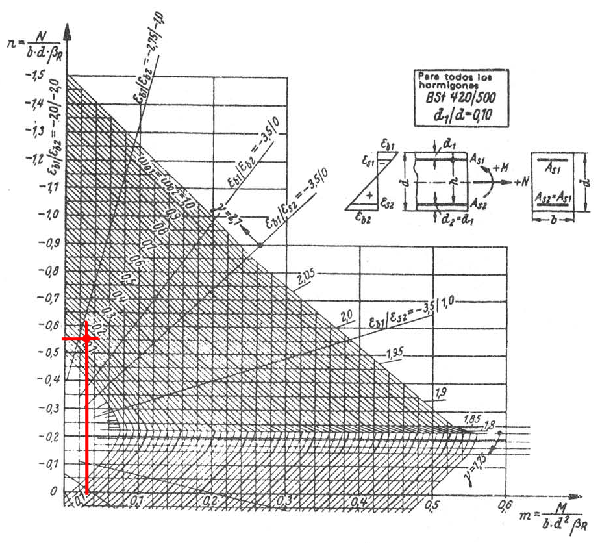
\includegraphics[scale = 0.9]{chapters/chapter_1/images/figura3.png}
     \caption{Diagrama de interacción $\frac{d_1}{d} = 0.10$)}
\end{center}
\end{figure}
Ingresando al diagrama de interacción con $m_{n}=0.033$, $n_{n}=0.56$ y $\frac{d_1}{d} = 0.10$ tenemos $\omega_{01} = \omega_{02} = 0.18$

\item \underline{Cuantía mecánica}
\begin{align*}
& \mu_{01} \text{ por cara} = \omega_{01} \cdot \frac{\beta_R}{\beta_S} = 0.18 \cdot \frac{175 \frac{Kg}{cm^2}}{4200 \frac{Kg}{cm^2}} = \framebox{0.0075} \text{ por cara}
\end{align*}

\item \underline{Armadura}

\begin{align*}
& As_{\text{ por cara}} = \mu_{01} \cdot b \cdot d = 0.0075 \cdot 35cm \cdot 35cm = \framebox{$9.19cm^2$} \text{ por cara}
\end{align*}
Adopto 3 barras $\phi$ 20 mm con $As_{\text{ por cara}}=\framebox{$9.42cm^2$}$\\
Adopto estribos $\phi$ 8 mm cada 20cm.\\

\item \underline{Verificación de Separaciones}\\
\\
Adopto s = 20 cm.\\
\[ s = 20cm \leq \left\{ \begin{array}{ll}
         12 \cdot db = 12 \cdot 2cm = 24cm \quad \surd &\\
         b = 35cm \quad \surd & \end{array} \right. \] 

\item \underline{Cuantía total $\mu$}

\begin{align*}
& \mu = \frac{A_s}{A_g} = \frac{2 \cdot 9.42cm^2}{35cm \cdot 35cm} = \framebox{0.015} \\
& \mu > \text{Cuantía mínima} \\
& 0.015 > 0.008 \quad \surd \text{ Verifica}
\end{align*}

\end{itemize}
\end{enumerate}